\documentclass{article}

\usepackage[a4paper,left=1in,right=1in,top=1in,bottom=1in,footskip=.25in]{geometry}
\usepackage{listings}
\usepackage{lipsum}
\usepackage{graphicx}
\usepackage{afterpage}
\usepackage{xcolor}
\usepackage{fancyhdr}
\usepackage{float}
\usepackage{helvet}
\usepackage{url}
\usepackage[toc,page]{appendix}
\usepackage[final]{pdfpages}
\usepackage[hidelinks]{hyperref}




\renewcommand{\familydefault}{\sfdefault}

\pagestyle{fancy}

\graphicspath{{./IMAGES/}}

\lstset{
	escapeinside={/*@}{@*/},
	language=Java,	
	basicstyle=\ttfamily\fontsize{8.5}{12},
	numbers=left,
	numbersep=2pt,    
	xleftmargin=2pt,
	frame=tb,
	columns=fullflexible,
	showstringspaces=false,
	tabsize=4,
	keepspaces=true,
	showtabs=false,
	showspaces=false,
	morekeywords={inline,public,class,private,protected,struct},
	captionpos=b,
	lineskip=-0.4em,
	aboveskip=10pt,
	extendedchars=true,
	breaklines=true,
	prebreak = \raisebox{0ex}[0ex][0ex]{\ensuremath{\hookleftarrow}},
	keywordstyle=\color[rgb]{0,0,1},
	commentstyle=\color[rgb]{0.133,0.545,0.133},
	stringstyle=\color[rgb]{0.627,0.126,0.941},
}

\title{USB/Bluetooth Media Controller\\Final Report}
\author{40056761\\SET09118\\Edinburgh Napier University}
\date{22-04-2016}
\makeatletter
\lhead{SET09118: Final Report}
\rhead{40056761}


\begin{document}
		
	\maketitle
	
	\section{Abstract}
		This document is the final report and a conclusion to the "USB/Bluetooth Media Controller" project started in February [Appendix \ref{IPP}] [Appendix \ref{Interim}]. The purpose of this project was to research, construct and evaluate a micro-controller based system and mobile application, that would allow a user to communicate with a media device via more intuitive methods.
				
	\newpage
		
	\pagenumbering{arabic}
		
	\tableofcontents
	
	\listoffigures
	
	\listoftables
	
	\lstlistoflistings
		
	\newpage
		
	\section{Introduction}
		\subsection{Background and Rational}
			\lipsum[1]
		
		\subsection{Aims and Deliverables}
			\lipsum[1]
	
	\section{Design}
		\subsection{Physical System Design}
			\lipsum[1]
			
			\begin{table}[h]
				\centering
				\caption{A usage table of the HID commands utilized by the media-controller}
				\label{my-label}
				\begin{tabular}{|r|r|r|}
					\hline
					\multicolumn{1}{|l|}{Usage ID} & \multicolumn{1}{l|}{Usage Name} & \multicolumn{1}{l|}{Usage Type} \\ \hline
					0xCD                           & Play/Pause                      & OSC                             \\
					0xB0                           & Play                            & OOC                             \\
					0xB1                           & Pause                           & OOC                             \\
					0xB3                           & Fast Forward                    & OOC                             \\
					0xB4                           & Rewind                          & OOC                             \\
					0xB5                           & Scan Next Track                 & OSC                             \\
					0xB6                           & Scan Previous Track             & OSC                             \\
					0xB7                           & Stop                            & OSC                             \\
					0xE2                           & Mute                            & OOC                             \\
					0xE9                           & Volume Increment                & RTC                             \\
					0xEA                           & Volume Decrement                & RTC                             \\ \hline
				\end{tabular}
			\end{table}
		
		\subsection{Mobile Application Design}
			\lipsum[1]

	\section{Implementation}
		\subsection{Micro-controller Implementation}
			\lipsum[1]
			
		\subsection{Mobile Application Implementation}
			\lipsum[1]
			
	\section{Results}
		\subsection{Achievements}
			\lipsum[1]
			
		\subsection{Recommendations}
			\lipsum[1]
			
	\section{Future Work}
		\lipsum[1]
	
	\section{Conclusion}
		\lipsum[1]
		
	\section{Evaluation of Achievement}
		\lipsum[1]
		
	\bibliographystyle{ieeetran}
	
	\bibliography{final}

	\newpage

	\begin{appendices}

		\section{Arduino Media-Controller Source Code}
			\lstinputlisting[caption = mediaController\_debounce.ino, nolol]{../../ARDUINO/mediaController_debounce/mediaController_debounce.ino}
			\newpage
			
		\section{Arduino Media Key Library}
			\lstinputlisting[title = Media.h, nolol]{../../ARDUINO/Media/Media.h}
			\newpage
			\lstinputlisting[title = Media.cpp, nolol]{../../ARDUINO/Media/Media.cpp}
			\newpage
			
		\section{Android Application Source code}
			\lstinputlisting[title = MainActivity.java, nolol]{../../ANDROID/MediaController/app/src/main/java/uk/co/sam/mediacontroller/MainActivity.java}
			\newpage
			
			\lstinputlisting[title = BluetoothHandler.java, nolol]{../../ANDROID/MediaController/app/src/main/java/uk/co/sam/mediacontroller/BluetoothHandler.java}
			\newpage
					
		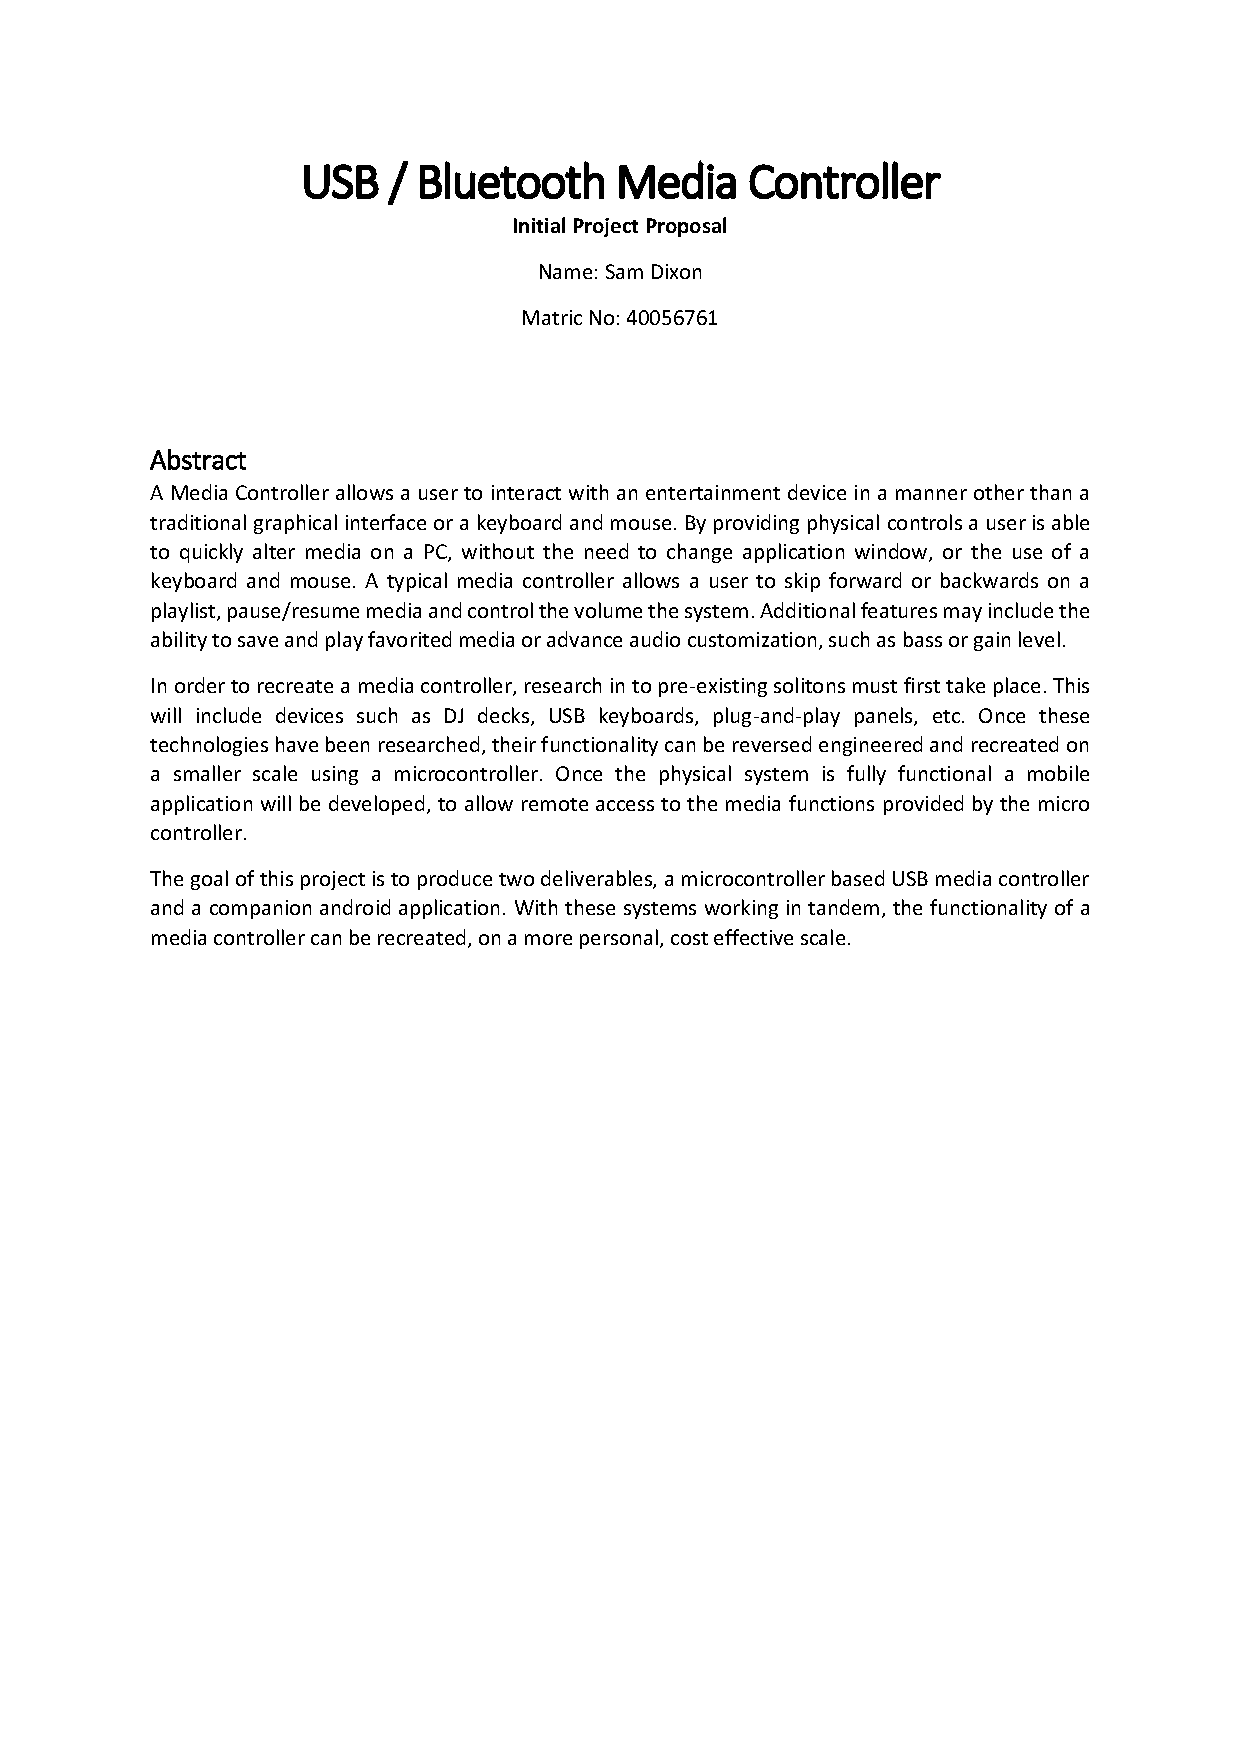
\includepdf[scale = 0.8, pages=1,pagecommand=\section{Initial Project Proposal}\label{IPP}]{../IPP/SET09118_IPP.pdf}
		\includepdf[scale = 0.8, pages=2-,pagecommand={}]{../IPP/SET09118_IPP.pdf}
		\newpage
	
		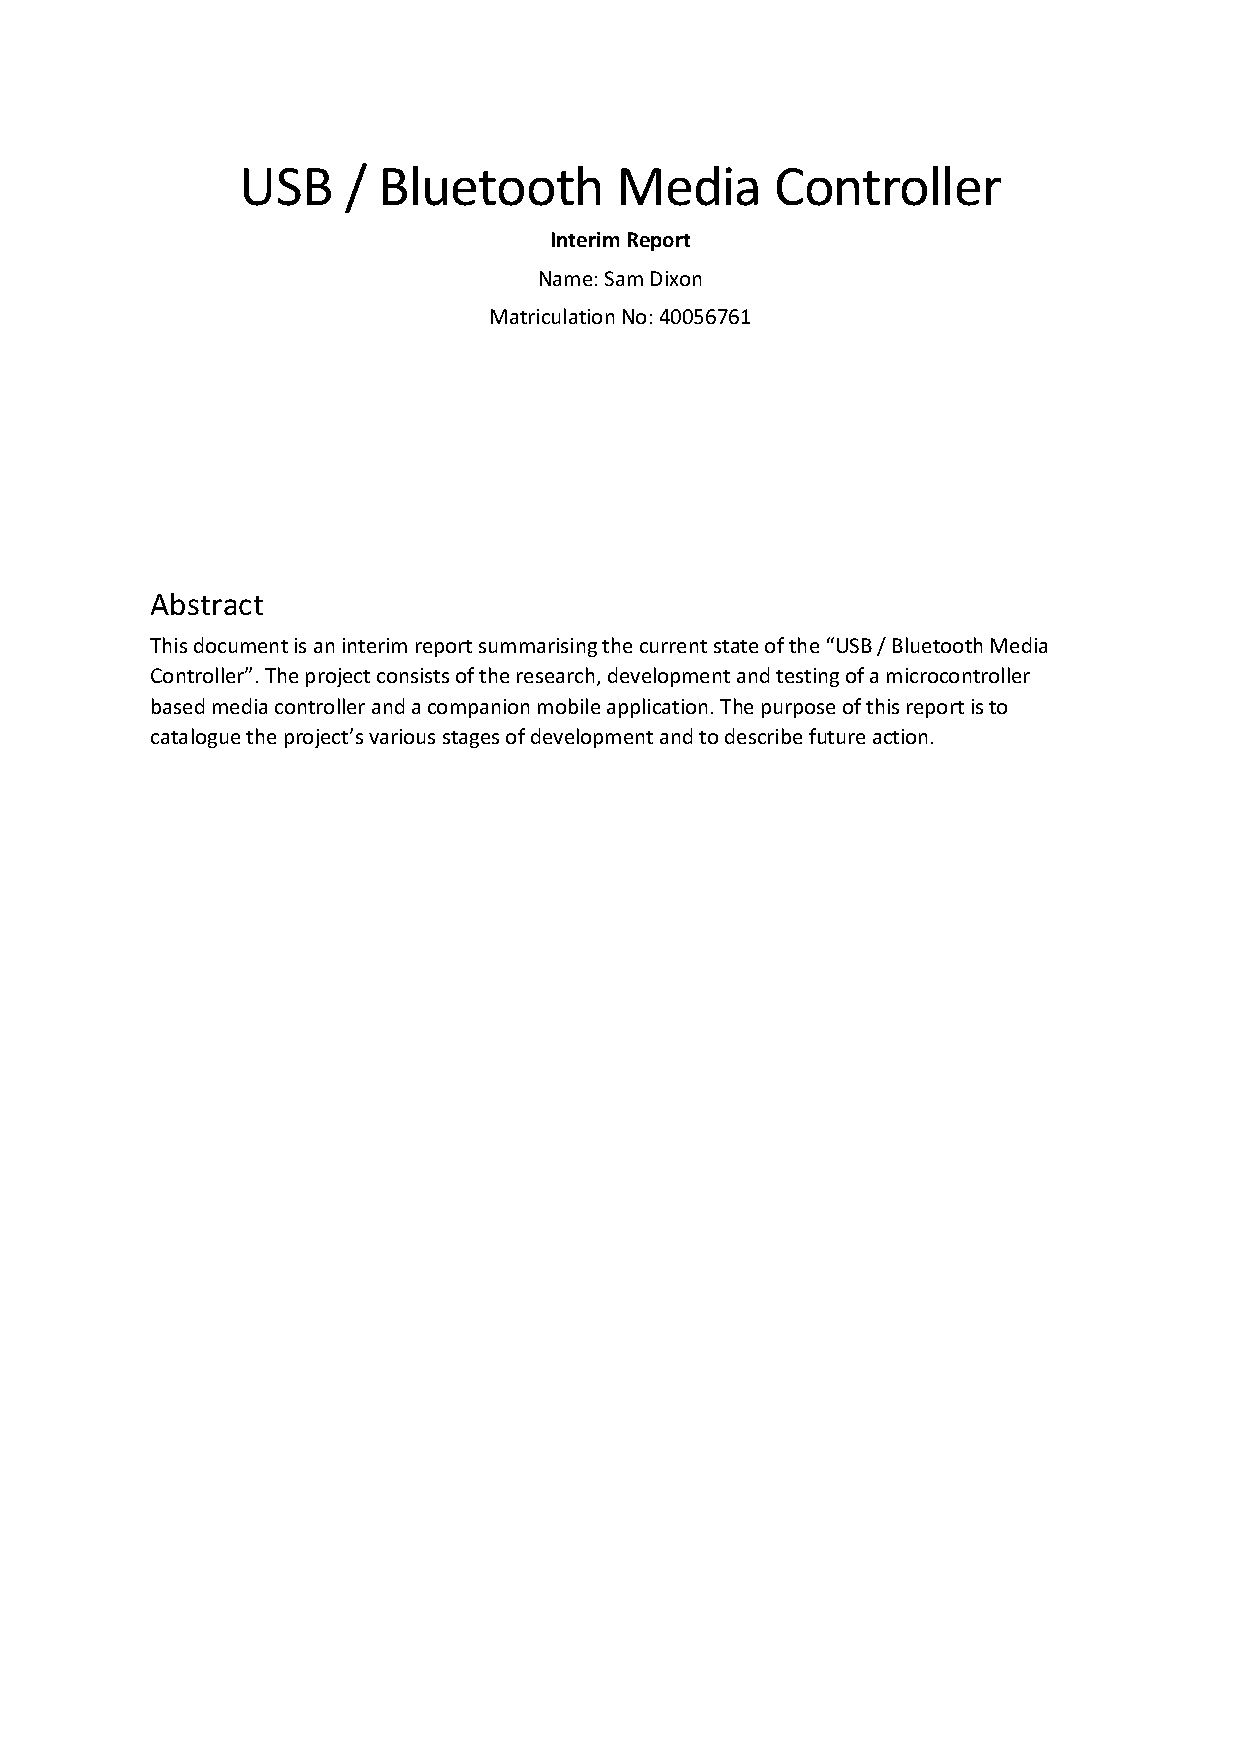
\includepdf[scale = 0.8, pages=1,pagecommand=\section{Interim Report}\label{Interim}]{../INTERIM/SET09118_INTERIM.pdf}
		\includepdf[scale = 0.8, pages=2-,pagecommand={}]{../INTERIM/SET09118_INTERIM.pdf}
		\newpage	

		 		
	\end{appendices}

\end{document}